\chapter{JT60-SA control design}

\section{Machine description}
\begin{figure}
	\centering
	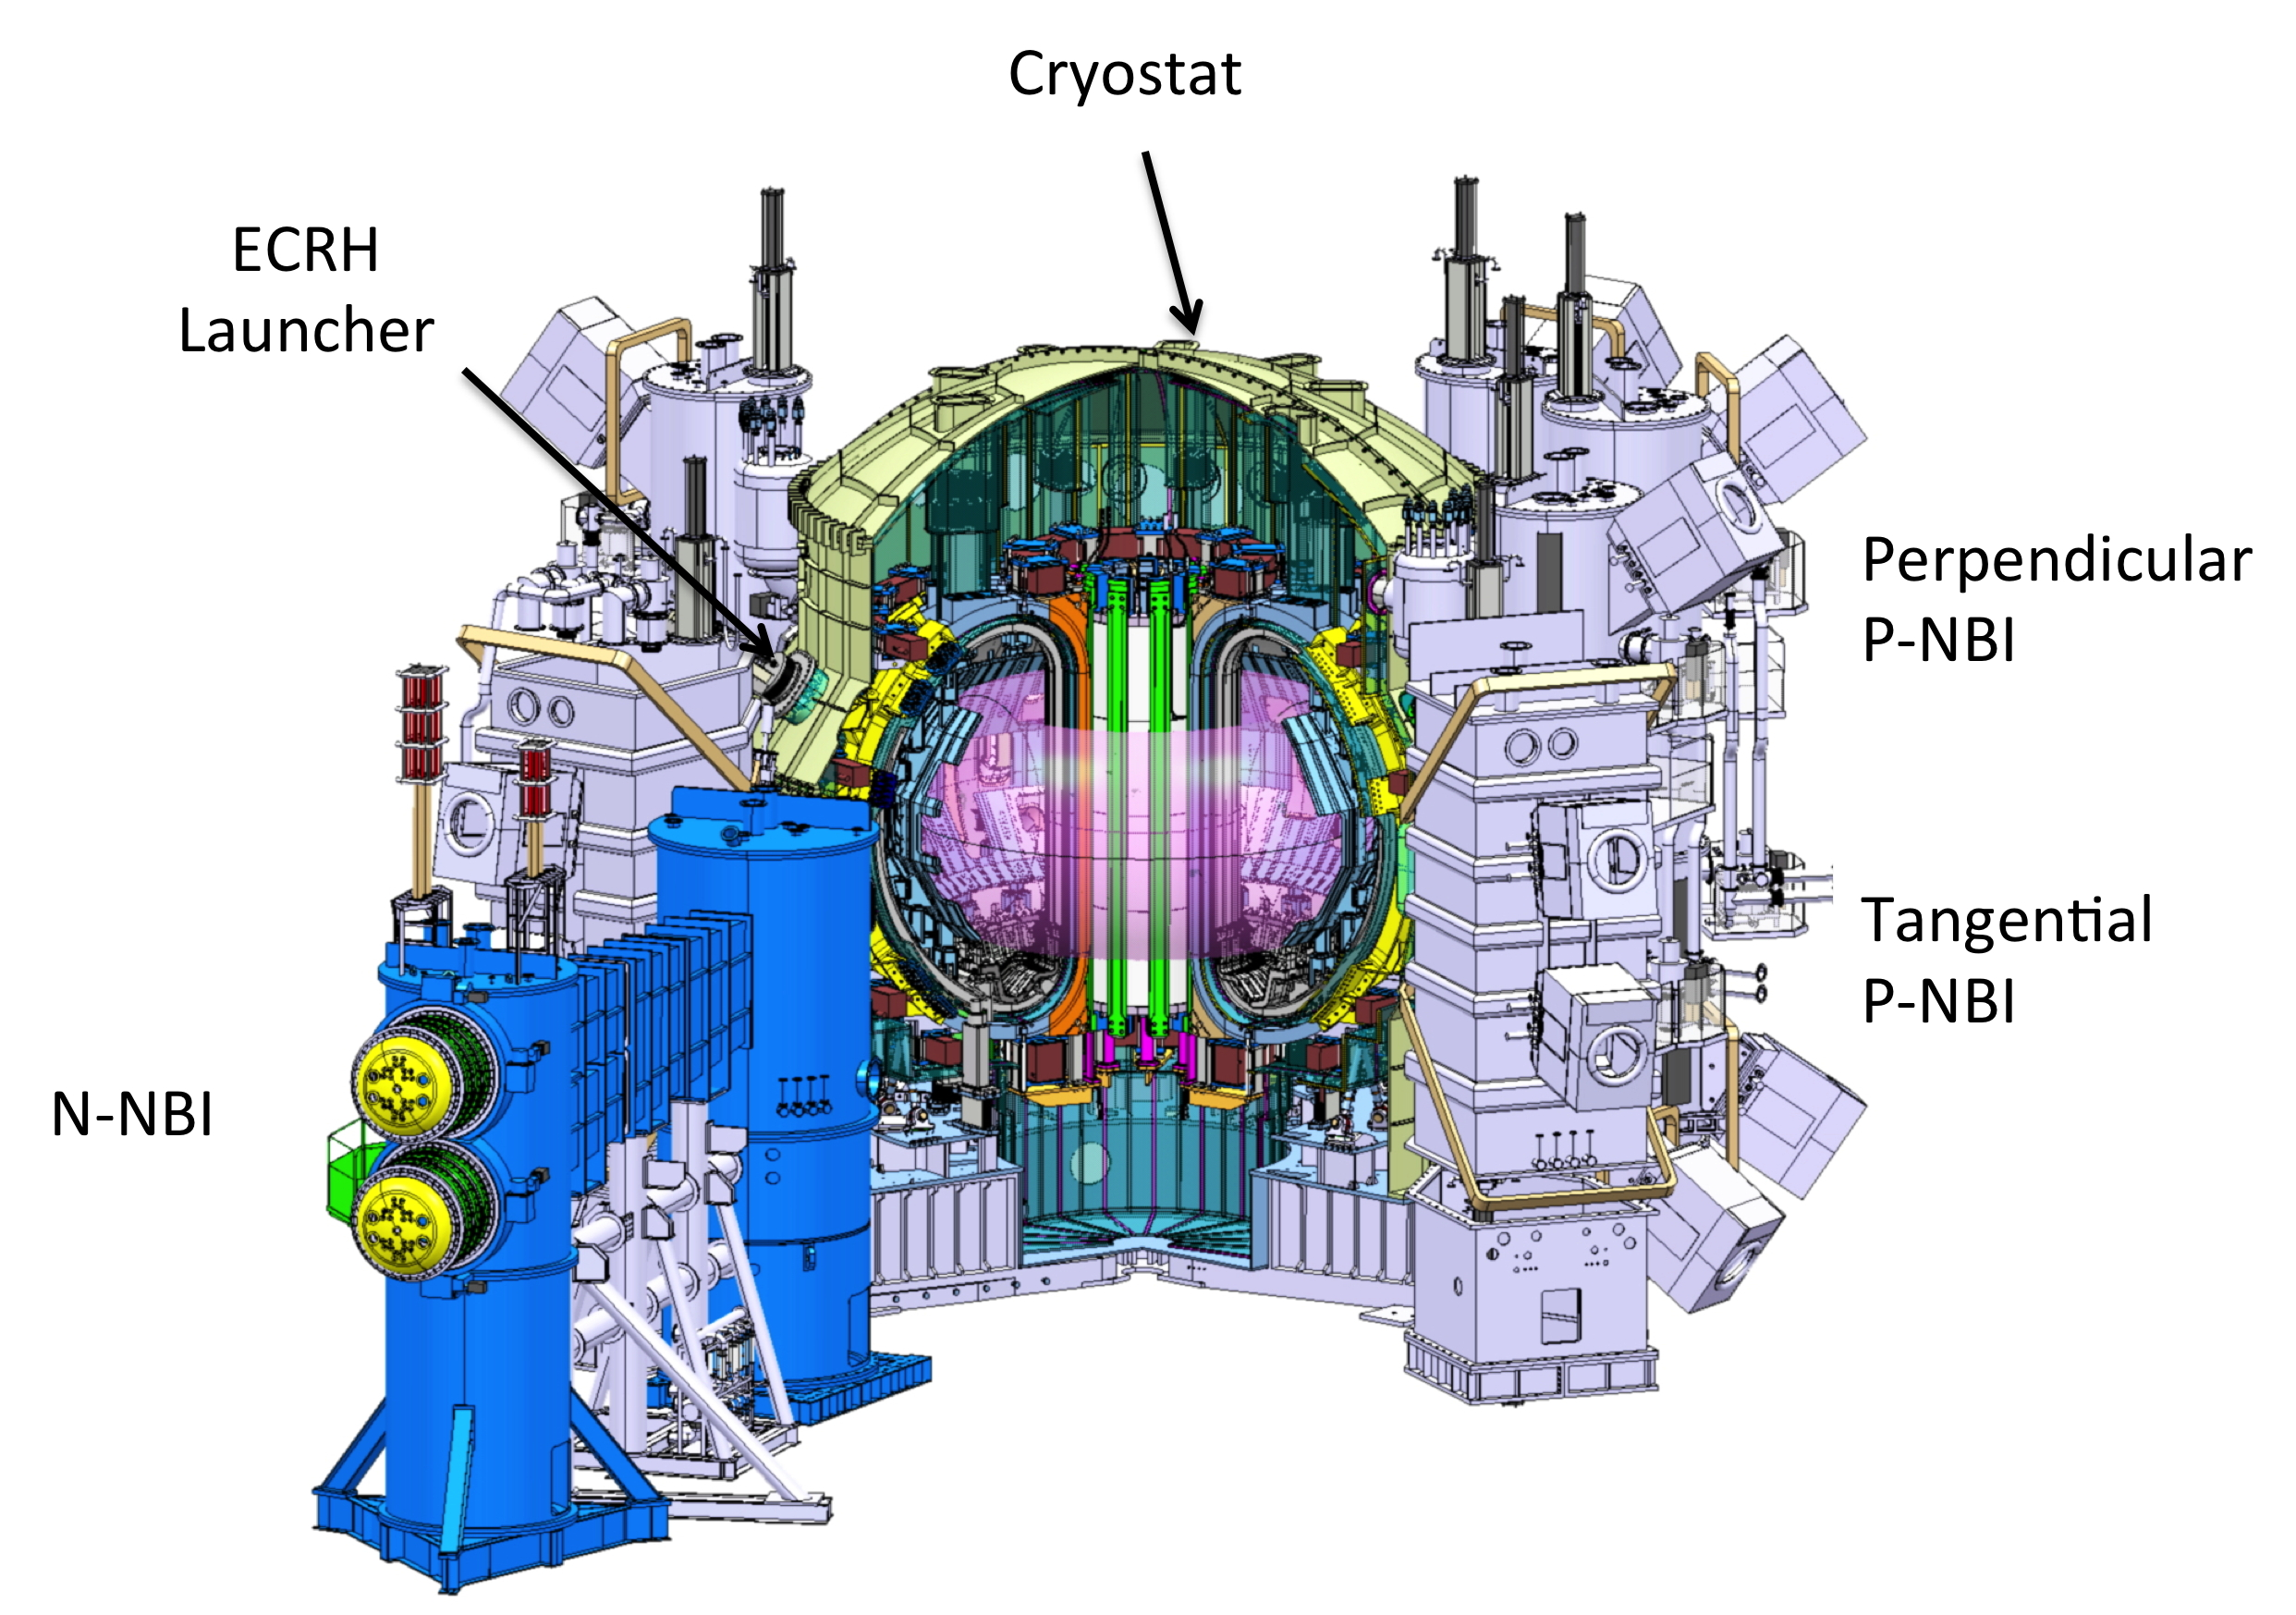
\includegraphics[width=0.80\textwidth]{Chp3/JT60SA.png}
	\label{JT60schm}
	\caption{JT60-SA tokamak configuration}
\end{figure}

\section{CREATE tools}
\section{Controller design}
\subsection{eXtreme Shape Controller}
\section{QST tools implementation}
\subsection{CCS}
\subsection{QST magnetic controller (FBC)}
QST magnetic controller calculates command values of active coil ccurrents/voltages from some information
\begin{equation}
I_{PF\_ref}(t+\Delta t) = I_{PF}(t_0)+M^\dagger_{PF}\left[G_{SP}\delta\Psi_s(t)+G_{SI}\int_{t_0}^{t}\delta\Psi_s(t)dt+G_{XP}\delta\Psi_X(t)+G_{XI}\int_{t0}^{t}\delta\Psi_x(t)dt\right]
\end{equation}

\begin{equation}
V_{com}=G_{vt}\left[M_{coil}\frac{(I_{coil\_ref}-I_{coil\_meas})}{dt}+ \frac{M_{plasma\_now} \cdot I_{p\_now} - M_{plasma\_ bfr} \cdot I_{p\_bfr}}{dt}\right]
\end{equation}

\begin{equation}
I_{FPPC\_ref}(t+\Delta t)=I_{FPPC}(t_0)+ M^\dagger_{FPPC}\left[G_{FP}\delta \Psi_{SF}(t) + G_{FD}\frac{d}{dt}\delta\Psi_{SF}(t) \right]
\end{equation}
\section{Simulation results}	

\subsection{ELM}
\subsection{Compound ELM}
\subsection{Minor Disruption}